\documentclass[11pt,letterpaper]{article}
\usepackage[margin=0.86in]{geometry}
\usepackage[T1]{fontenc}
\usepackage[utf8]{inputenc}
\usepackage{lmodern}
\usepackage{xcolor}
\usepackage{tabularx,booktabs,array,longtable}
\usepackage{enumitem}
\usepackage{hyperref}
\usepackage{fancyhdr}
\usepackage{lastpage}
\usepackage{titlesec}
\usepackage{amsmath,amssymb}
\usepackage{microtype}
\usepackage{needspace}
\usepackage{ragged2e}
\usepackage{graphicx}
\newcommand{\todo}[1]{\textcolor{red}{\textbf{[TODO: #1]}}}
\definecolor{navy}{HTML}{19334C}
\definecolor{teal}{HTML}{236B82}
\definecolor{soft}{HTML}{EFF5F7}
\definecolor{muted}{HTML}{52616B}
\hypersetup{colorlinks=true,linkcolor=teal,urlcolor=teal}
\titleformat{\section}{\Large\bfseries\color{navy}}{\thesection.}{0.6em}{}
\titleformat{\subsection}{\large\bfseries\color{navy}}{\thesubsection}{0.6em}{}
\titleformat{\subsubsection}{\normalsize\bfseries\color{navy}}{\thesubsubsection}{0.6em}{}
\titlespacing*{\section}{0pt}{15pt}{6pt}
\titlespacing*{\subsection}{0pt}{10pt}{4pt}
\setlength{\parindent}{0pt}
\setlength{\parskip}{4.5pt}
\setlength{\headheight}{15pt}
\renewcommand{\arraystretch}{1.16}
\setlist[itemize]{topsep=3pt,itemsep=2pt,leftmargin=1.4em}
\setlist[enumerate]{topsep=3pt,itemsep=2pt,leftmargin=1.5em}
\pagestyle{fancy}
\fancyhf{}
\fancyhead[L]{\small\color{muted} Applied Machine Learning \textbar{} Cornell Tech}
\fancyhead[R]{\small\color{muted} Human or AI?}
\fancyfoot[C]{\small\color{muted} Page \thepage\ of \pageref{LastPage}}
\renewcommand{\headrulewidth}{0.3pt}
\newcommand{\placeholder}[1]{\par\noindent\textcolor{teal}{\textit{[Your response: #1]}}\par\vspace{0.3em}}
\newcommand{\figplaceholder}[1]{\par\noindent\fcolorbox{teal}{soft}{\parbox[c][1.15in][c]{0.94\linewidth}{\centering\textcolor{muted}{Insert #1 here}}}\par}
\newcommand{\question}[2]{\needspace{4\baselineskip}\par\addvspace{0.45em}\noindent\textbf{#1}\quad #2\par\nobreak\vspace{0.1em}}
\newcommand{\smallnote}[1]{{\small\color{muted}#1}}
\newcolumntype{Y}{>{\RaggedRight\arraybackslash}X}
\begin{document}
\thispagestyle{empty}
\vspace*{0.2in}
{\color{teal}\bfseries CORNELL TECH \textbar{} APPLIED MACHINE LEARNING}\par
\vspace{0.15in}
{\Huge\bfseries\color{navy} Human or AI?}\par
\vspace{0.07in}
{\LARGE\color{navy} Kaggle Competition \&  Report Template}\par
\vspace{0.17in}

\textbf{Report Template: }\href{https://www.overleaf.com/project/6ae1fc85355dcf680137d898/share#f2777b20d3adeeecfac9096f78008e2f8daa0ff4be43de3b}{TEMPLATE}

\textbf{Github Repository Template: }\href{https://github.com/sekhari/human-or-ai-submissions}{REPO}

\textbf{Welcome to the competition!} Your task is to build a machine learning classifier that predicts whether a passage was written by a human or generated by an AI model. You will use a labeled training set, an additional unlabeled set, and a held-out Kaggle test set. The aim is not just a high leaderboard score: we want you to compare methods, design careful experiments, understand generalization, and explain what your results actually show.

You are encouraged to try several approaches. A well-tested logistic regression or support vector machine is just as legitimate as a neural network. The project is designed to be approachable on a laptop; a GPU is \emph{not required} for full credit.

\vspace{0.06in}
\begin{tabularx}{\linewidth}{@{}>{\bfseries}p{1.58in}Y@{}}
Team / members & Chris Viets, Yuchen Gao, Daniel Xing \\
Kaggle team name & \texttt{Group\_Number\_19} \\
GitHub PR URL & \todo{PR link to sekhari/human-or-ai-submissions} \\
\end{tabularx}
\vspace{0.06in}
\subsection*{Your data}
\begin{tabularx}{\linewidth}{@{}lrrY@{}}
\toprule
\textbf{File} & \textbf{Rows} & \textbf{Labels} & \textbf{Purpose} \\
\midrule
\texttt{train.csv} & 10,000 & Visible & Supervised model development: 5,000 human (0), 5,000 AI (1) \\
\texttt{unlabeled.csv} & 3,000 & Hidden & Optional input for semi-supervised methods; required experiment \\
\texttt{test.csv} & 3,000 & Hidden & Predict the probability of AI authorship for Kaggle \\
\texttt{train\_starter\_2000.csv} & 2,000 & Visible & Convenient subset of \texttt{train.csv} for quick experiments \\
\bottomrule
\end{tabularx}

\smallnote{The starter data is a subset, not 2,000 additional labeled examples. Passages are approximately 75--350 words, with mean length near 210 words.}

\subsection*{How the test set works}
The test set mixes familiar and unfamiliar writing domains and AI generators, and includes some adversarially modified AI-written passages. You will \emph{not} receive labels, source model names, domain labels, or difficulty memberships for individual test examples. Submit a probability in $[0,1]$ for each test ID, where 1 means AI-generated. Kaggle evaluates submissions using \textbf{area under the ROC curve (AUROC)}. The \textbf{public leaderboard} covers 900 examples (30\%); the \textbf{private leaderboard} covers 2,100 (70\%) and determines the final competition performance score.


\vfill
\newpage
\section{Competition rubric and submission instructions}
\begin{tabularx}{\linewidth}{@{}Y>{\raggedleft\arraybackslash}p{0.85in}@{}}
\toprule \textbf{Component} & \textbf{Points}\\ \midrule
Kaggle private leaderboard performance & 25 \\
Model comparison and selection & 15 \\
Effect of training data size & 10 \\
Learning from unlabeled data & 5 \\
Generalization and error analysis & 20 \\
Open-ended improvements and insights & 15 \\
Code submission and GitHub PR history & 10 \\
\midrule \textbf{Total} & \textbf{100} \\ \bottomrule
\end{tabularx}

\textbf{How to use this document.} Complete the response fields and tables below; insert plots where requested. Keep your answers concise, specific, and supported by actual experiments. Points appear in brackets beside each question; no separate writing-quality grade is assigned.

\textbf{How credit is awarded.} We grade the \emph{quality of the experimental method, evidence, and interpretation}, not whether a proposed idea succeeds. \textbf{Negative results can also earn full credit} when the comparison is valid, the results are reported accurately, and the conclusions are thoughtful. For each question, make clear what you tried, what you measured, and what you learned. Do not invent scores or results.

\textbf{Submit three items:} (1) final Kaggle submission; (2) this completed report as PDF; (3) one GitHub PR link in the course repository, with runnable code, instructions and meaningful commit history. Include the PR link on the title page. Confirm upload locations and deadline time on the course site. The template for the repository is \href{https://github.com/sekhari/human-or-ai-submissions}{here}

\textbf{Compute and models.} Use models and pipelines that you can run and reproduce. Laptop-friendly training is strongly recommended; use of more expensive methods is allowed but not required for full credit. Do not use external LLM APIs to directly label or predict the competition test passages. Use only the supplied labeled dataset for supervised labels; allowed pretrained weights and AI-assisted development should be disclosed.

\textbf{Validation.} For the required controlled experiments, reserve a fixed stratified \textbf{2,000-row validation set} from \texttt{train.csv}, leaving up to 8,000 rows for training. Use the \emph{same} held-out validation set for comparisons and do not tune on test labels. You may retrain your final Kaggle model on all 10,000 labeled examples after selecting your approach. Where possible, document seeds and avoid source/near-duplicate leakage.

\textbf{Kaggle grading (25 points).} Final performance will use the private AUROC, not leaderboard rank. The intended continuous rule is $25\,\mathrm{clip}((A-0.50)/(T-0.50),0,1)$, where $A$ is your private AUROC and $T$ is the announced full-credit threshold. A provisional value of $T=0.90$ is under consideration; the instructors will confirm the fixed threshold before launch. A reference word TF-IDF and logistic regression baseline achieves approximately 0.868 private AUROC.

\section{Team information and model summary}
\question{Q0.1 [0 points].}{List team members and their main contributions.}
\begin{itemize}
\item \textbf{Chris Viets (cv329)}: \todo{contributions, e.g.\ TF-IDF baselines, style features, LightGBM stack, layout diagnostics}
\item \textbf{Daniel Xing}: \todo{NetID and contributions}
\item \textbf{Yuchen Gao (yg673)}: CatBoost line (v1--v4): leave-topic-cluster-out validation for the train/test genre shift, additional style features, GPT-2 and Qwen3.5 language-model features (run on the lab GPU cluster), self-training with unlabeled and test text, RoBERTa and classifier comparisons, the fixed-split experiments in Sections~1--4, and the final submission.
\end{itemize}
\question{Q0.2 [0 points].}{Summarize your final approach in 3--5 sentences. What is the overall pipeline from raw text to probability?}
Each passage is turned into 193 numbers: 126 hand-crafted style features (layout and blank lines, sentence-length burstiness, punctuation, vocabulary rarity, compressibility, rhyme), the out-of-fold score of a TF-IDF (word 1--3 + character 3--5 grams) logistic regression, 35 token-probability statistics from frozen GPT-2 small/medium (perplexity, log-probability spread, Fast-DetectGPT), and 31 Binoculars-style features from frozen Qwen3.5-2B Base/Instruct. A CatBoost classifier (3 seeds averaged) maps these to $P(\text{AI})$. One round of self-training then adds confidently pseudo-labeled passages ($P>0.95$ or $P<0.05$) from \texttt{unlabeled.csv} and \texttt{test.csv} and refits. The final submission rank-averages this model (weight 0.9) with a fine-tuned RoBERTa-base classifier (weight 0.1). Models were selected with leave-one-topic-cluster-out validation, because the test set contains far more poetry/fiction than train.
\question{Q0.3 [0 points].}{Record your final scores (enter private score only once it is revealed).}
\begin{tabularx}{\linewidth}{@{}Yp{1.8in}@{}}\toprule Metric & Your score \\ \midrule Validation AUROC, fixed 2,000-row split (final blend) & 0.99928 \\ Validation AUROC, leave-cluster-out (final blend) & 0.99953 \\ Kaggle public AUROC (final blend) & 0.99162 \\ Kaggle private AUROC & \todo{after reveal} \\ \bottomrule\end{tabularx}

\newpage
\section{Model comparison and selection (15 points)}
\textbf{Learning goal:} demonstrate sensible representation choices, comparisons of at least three approaches, appropriate hyperparameter selection, and evidence-based selection of the final classifier.

\question{Q1.1 [3 points].}{How did you preprocess and represent the text? Specify tokenization, normalization, word/character features or embeddings, and any feature extraction choices. Why?}
We keep the raw text, including case, whitespace and newlines, because layout is informative (66\% of AI training texts contain a blank line, versus 17 of 5,000 human texts). Four representations are combined: (i) TF-IDF on lower-cased word 1--3-grams (min\_df 2) and case-sensitive character 3--5-grams (min\_df 3, 300k features), binary tf and smoothed idf, fed to a logistic regression whose cross-fitted score becomes one feature; (ii) 126 style features computed with regex tokenization (blank lines and newline rate, sentence-length mean/variance, punctuation and capitalization rates, type--token ratio, word rarity from \texttt{wordfreq} Zipf frequencies, zlib compression ratio, line-end rhyme); (iii) per-token log-probability, entropy and rank statistics from frozen GPT-2 small/medium (BPE, first 512 tokens); (iv) Binoculars and cross-model scores from frozen Qwen3.5-2B Base and Instruct. Why: n-grams capture wording but are topic-bound, whereas (ii)--(iv) measure style and predictability, which should transfer to the unseen genres in test.
\question{Q1.2 [5 points].}{Which \textbf{three or more} modeling approaches did you try? Keep the labeled validation partition fixed across models.}
\begin{tabularx}{\linewidth}{@{}p{1.24in}Yrrr@{}}\toprule
Model & Text representation & Train AUROC & Val. AUROC & Train time \\ \midrule
TF-IDF + logistic regression ($C=30$) & word 1--3 + char 3--5-gram TF-IDF & 1.0000 & 0.97149 & 15 s \\
LightGBM (team baseline) & 53 style features + TF-IDF/LR score & 0.99993 & 0.99926 & 3 s \\
CatBoost (v2) & 126 style features + TF-IDF/LR score & 0.99988 & 0.99874 & 3 s \\
CatBoost (v4 features) & 126 style + TF-IDF/LR score + 35 GPT-2 + 31 Qwen3.5 & 0.99997 & 0.99925 & 6 s$^\dagger$ \\
MLP 256--128 & same 193 inputs, quantile-normalized & 0.99996 & 0.99900 & 1 s \\
RoBERTa-base (fine-tuned) & raw text, byte-level BPE, 512 tokens & 0.99951 & 0.99928 & 9 min (GPU) \\
\bottomrule\end{tabularx}
\smallnote{``TF-IDF/LR score'' = the out-of-fold probability from the TF-IDF + logistic regression model in the first row, used as one input feature. Fixed validation set: fold 0 of a stratified 5-fold split of \texttt{train.csv} (seed 20261109; 1,000 human + 1,000 AI); all models trained on the remaining 8,000 rows. $^\dagger$Plus a one-off GPU cost to compute the LM features for all 16,000 texts: $\sim$18 min (GPT-2, RTX 2080 Ti) and $\sim$24 min (Qwen3.5, RTX A6000). RoBERTa: 2 epochs, one RTX 2080 Ti (Appendix A.3).}
\question{Q1.3 [4 points].}{For at least \textbf{two} approaches, which hyperparameters and candidate values did you try? How did you select the final settings without using Kaggle test labels?}
\begin{tabularx}{\linewidth}{@{}p{1.18in}Yp{1.38in}@{}}\toprule Model & Parameters/values searched & Chosen setting \\ \midrule
CatBoost (v4 features) & depth $\{4,6,8\}$ $\times$ learning rate $\{0.03, 0.05, 0.1\}$; iterations by early stopping (patience 150, max 1,500) & depth 6, lr 0.05 (all 9 within 0.9985--0.9992 inner AUROC) \\
MLP (v4 features) & hidden layers $\{(128), (256,128)\}$ $\times$ L2 $\alpha \in \{10^{-4}, 10^{-3}, 10^{-2}\}$ & (256,128), $\alpha=10^{-4}$ (inner 0.99953) \\
Logistic regression (TF-IDF) & $C \in \{0.3, 1, 3, 10, 30\}$, tf/idf schemes, n-gram ranges (team sweep) & $C=30$, binary tf \\
\bottomrule\end{tabularx}
Every choice was made on data inside the 8,000-row training partition: we split it 80/20 (stratified) and scored each setting on the inner 20\%, which also served as the early-stopping set. The 2,000-row validation set and Kaggle labels were never used for selection. The CatBoost grid is flat: the best inner setting (depth 4, lr 0.1, 0.99925) differs from the others by less than 0.0008, so we re-checked the candidates under the leave-cluster-out protocol of Q1.4 (training labels only): depth 6 / lr 0.05 scores 0.99906 (0.99932 with self-training), depth 4 / lr 0.1 0.99901 (0.99930) and depth 6 / lr 0.1 0.99919 (0.99939). These differences are at most 0.0002, about the size of seed-to-seed variation, so we kept depth 6 / lr 0.05. For the MLP the inner ranking picked (256,128) with weak regularization.
\question{Q1.4 [3 points].}{Which approach did you choose for your final submission? Explain using validation performance, computational cost and/or stability. If you later changed the model, explain why.}
We chose CatBoost on the v4 features with self-training, rank-blended with a fine-tuned RoBERTa-base (weight 0.1). RoBERTa is the best single model on the fixed random split (0.99928), but only 0.9952 under leave-cluster-out, i.e.\ it is strong on familiar genres and weak on new ones, so it gets a small weight. On the fixed random split the feature-based models are tied at 0.999 (the team LightGBM equals v4 CatBoost), so this split cannot rank them; yet their public scores were 0.9754 and 0.9915. The reason is a genre shift: k-means topic clusters show poetry/fiction is 35.8\% of test but 1.5\% of train. We therefore also validated with leave-one-topic-cluster-out (LCO) CV weighted to the test cluster mix. Under LCO with identical features, CatBoost scores 0.99906, MLP 0.99886, extra trees 0.99843, logistic regression 0.99841, random forest 0.99795 and LightGBM 0.99399 (LightGBM drops on the held-out poetry cluster). CatBoost was also stable across hyperparameters and seeds and trains in seconds once the LM features are cached. We moved from the team LightGBM to CatBoost v2 (public 0.9788), then added GPT-2 (0.9887) and Qwen3.5 features (0.9915), each step chosen by its LCO gain. Finally, a 10\% RoBERTa rank blend raised LCO AUROC from 0.99939 to 0.99953 (RoBERTa alone: 0.9952) and the public score to 0.99162; it is the final submission. The blend gain is small and its weight was chosen on the same out-of-fold predictions, but it was consistent between LCO and the leaderboard.

\section{Effect of training data size (10 points)}
\textbf{Learning goal:} understand the effect of the number of labeled examples on fitting and generalization. This is an empirical exercise; no formal sample-complexity theory is required.

\question{Q2.1 [4 points].}{Choose one model configuration. Train it with 500, 1,000, 2,000, 5,000 and 8,000 examples sampled from your 8,000-row training partition. Keep the same validation set and hyperparameters.}
\begin{tabularx}{\linewidth}{@{}rrrY@{}}\toprule Training rows & Training AUROC & Validation AUROC & Notes (optional) \\ \midrule
500 & 0.99798 & 0.98873 & TF-IDF + LR alone: 0.910 \\
1,000 & 0.99877 & 0.99527 & TF-IDF + LR alone: 0.935 \\
2,000 & 0.99998 & 0.99883 & TF-IDF + LR alone: 0.952 \\
5,000 & 0.99998 & 0.99903 & TF-IDF + LR alone: 0.964 \\
8,000 & 0.99997 & 0.99925 & TF-IDF + LR alone: 0.971 \\
\bottomrule\end{tabularx}
\smallnote{Configuration: CatBoost on the v4 features, fixed hyperparameters (depth 6, lr 0.05, early stopping on 20\% of the subsample). Subsamples are stratified draws from the 8,000-row training partition; the TF-IDF/LR feature is refit (cross-fitted) on each subsample.}
\question{Q2.2 [3 points].}{Insert a plot of training and validation AUROC versus training-set size.}
\begin{center}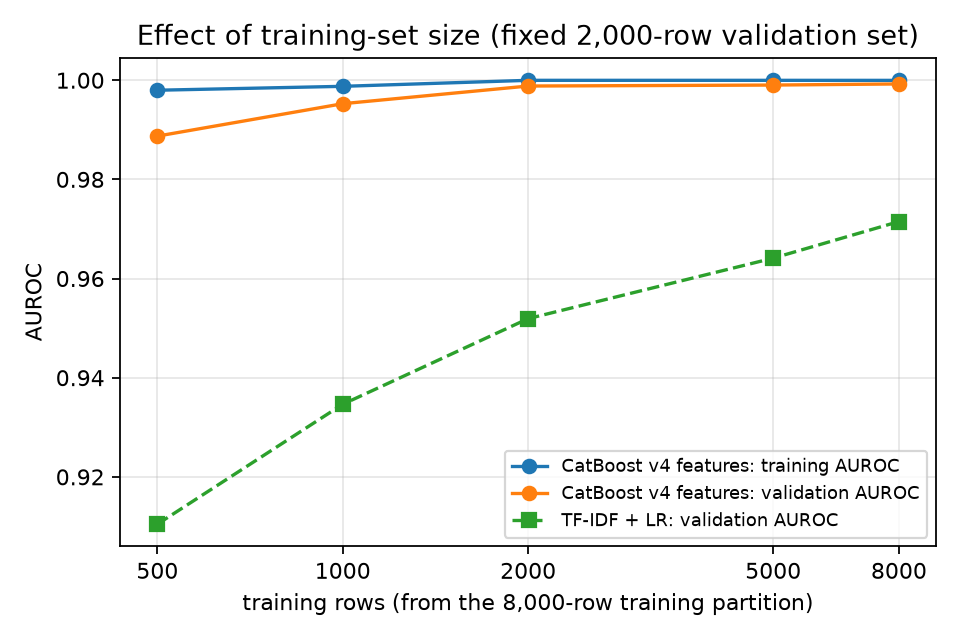
\includegraphics[width=0.78\linewidth]{learning_curve_fixed_val.png}\end{center}
\question{Q2.3 [3 points].}{What does the curve suggest about overfitting, underfitting, and the value of more labeled examples?}
With 500 rows the model overfits mildly: training AUROC is 0.998 but validation 0.989 (gap 0.009), and early stopping keeps only a few trees. The gap shrinks steadily and is 0.0007 at 8,000 rows; validation AUROC is essentially flat after 2,000 rows (0.9988 to 0.9993), so the feature model is not underfitting and more in-distribution labels would add little. The TF-IDF logistic regression behaves differently: it fits the training set perfectly at every size but its validation AUROC is still rising at 8,000 rows (0.910 to 0.971), so the high-dimensional n-gram model is data-hungry and would benefit from more labels. The real limit for our final model is not label count but distribution shift (Section 4): more labels of the same genres would not fix errors on unseen genres.

\section{Learning from unlabeled data (5 points)}
\textbf{Learning goal:} test whether the additional 3,000 unlabeled passages help.
\question{Q3.1 [2 points].}{Describe one method that uses \texttt{unlabeled.csv} (e.g., self-training, confidence-based pseudo-labeling, clustering, or feature learning). How did you prevent validation-label leakage?}
Confidence-based self-training. A CatBoost teacher (v4 features) is trained on the 8,000 training rows and scores the 3,000 passages of \texttt{unlabeled.csv}. Passages with $P>0.95$ or $P<0.05$ receive hard pseudo-labels (2,878 of 3,000; 49\% AI) and are added with weight 1; a student model is refit on labeled + pseudo-labeled rows and evaluated. Leakage control: the 2,000 validation rows are never in the teacher's training data or in the pseudo-label pool; the TF-IDF/LR feature for unlabeled rows comes from the model fit on the training partition only; early stopping uses an inner split of the training rows. We also tried thresholds 0.90 and 0.98.
\question{Q3.2 [2 points].}{Compare against a supervised baseline under the same held-out validation protocol.}
\begin{tabularx}{\linewidth}{@{}Yp{1.5in}@{}}\toprule Method & Validation AUROC \\ \midrule Supervised only & 0.99925 \\ With unlabeled data (threshold 0.95) & 0.99904 \\ \quad threshold 0.90 / 0.98 & 0.99906 / 0.99895 \\ \midrule \multicolumn{2}{@{}l}{\textit{Leave-cluster-out protocol (held-out genre), weighted AUROC:}} \\ Supervised only & 0.99884 \\ + \texttt{unlabeled.csv} & 0.99897 \\ + target (held-out) texts & 0.99922 \\ \bottomrule\end{tabularx}
\question{Q3.3 [1 point].}{Did it help? Give a concrete, evidence-based explanation (including possible noise in pseudo-labels).}
Not on the fixed split (about $-0.0002$). Pseudo-label noise is low: on validation rows where the teacher is equally confident (97\% of them), it is 99.85\% correct, so roughly 4 of the 2,878 pseudo-labels are wrong. The problem is redundancy: a TF-IDF classifier trained to tell train from test calls 7\% of train, 45\% of test, but only 11\% of \texttt{unlabeled.csv} ``test-like'', so the unlabeled passages come from the training distribution and their confident labels repeat what the labeled data already says. When the held-out genre is new (LCO), they help slightly, and self-training on the target texts themselves helps most, which is why the final model also pseudo-labels \texttt{test.csv} (texts only, no labels).

\newpage
\section{Generalization and error analysis (20 points)}
\textbf{Learning goal:} characterize how well the selected model generalizes and where it fails. Use \textbf{labeled validation data}; hidden test labels and hidden domain/generator information are unavailable.

\question{Q4.1 [5 points].}{Compare training and validation AUROC for your final selected model. Is there a gap? What explanations are plausible?}
The final model is the rank blend $0.9\times$CatBoost (v4 features, 3 seeds, self-training on \texttt{unlabeled.csv} + \texttt{test.csv} texts) $+\,0.1\times$RoBERTa-base, both refit on the same 8,000-row partition. Training AUROC is 0.99998 and validation AUROC 0.99928 (CatBoost part: 0.99999 / 0.99909; RoBERTa part: 0.99951 / 0.99928). The train--validation gap (0.0007) is small: boosted trees nearly memorize the training rows, and the remaining validation errors are rare, atypical passages, so the model generalizes well \emph{within} the training distribution. The much larger gap is between validation and the public leaderboard (0.999 vs 0.992). Plausible explanations: test over-represents genres that are rare in train (poetry/fiction 35.8\% vs 1.5\%), contains AI generators and adversarially edited passages absent from train, and likely contains human texts with blank lines, which are almost absent from train. RoBERTa illustrates the same effect: it ties for best on this random split but scores 0.9952 when the genre is held out.
\question{Q4.2 [5 points].}{Evaluate performance over at least three text-length bins (define the bins), or another observable subgroup available in your data. Explain why you chose the grouping.}
\begin{tabularx}{\linewidth}{@{}Yrrrr@{}}\toprule Subgroup / bin & Count & Val.\ AUROC (blend) & CatBoost alone & Errors$^\ddagger$ \\ \midrule
Short: $<150$ words & 384 & 0.99989 & 0.99978 & 3 \\
Medium: 150--250 words & 1,033 & 0.99964 & 0.99955 & 3 \\
Long: $>250$ words & 583 & 0.99869 & 0.99817 & 5 \\ \midrule
No blank line & 1,324 (25\% AI) & 0.99785 & 0.99728 & 11 \\
Has a blank line & 676 (99\% AI) & 1.00000 & 1.00000 & 0 \\ \bottomrule\end{tabularx}
\smallnote{$^\ddagger$The blend outputs a rank score, not a probability, so errors are counted at the score threshold that labels the same share of passages AI as CatBoost does at $P=0.5$ (blend score 0.5055): 1 false positive and 10 false negatives.}
Length bins test whether short passages carry too little signal; the blank-line split tests how much the model relies on the strongest layout cue. Contrary to our expectation, long passages are the hardest (0.9987), not short ones; the long errors are mostly AI encyclopedic texts (biographies, history) whose style is closest to the human Wikipedia articles in train, so length seems to act through genre rather than through signal strength. The blank-line split is far more informative: with a blank line the task is trivial in this data (99\% AI), and all 11 errors come from passages without one. Any test passage that breaks the ``blank line $\Rightarrow$ AI'' rule is therefore a likely failure.
\question{Q4.3 [5 points].}{Analyze at least \textbf{five false positives and five false negatives} from your held-out validation set. Provide example IDs, predicted probabilities, and short failure hypotheses. Do not paste full passages unless essential.}
\begin{tabularx}{\linewidth}{@{}p{0.45in}p{0.5in}p{1.15in}Y@{}}\toprule ID & Error type & Score (CatBoost / RoBERTa $P$) & Possible reason \\ \midrule
3326 & FP & 0.509 (0.85 / 1.00) & Polished, superlative movie review (``Academy Award winning war epic''); both models read the fluent generic praise as LLM prose \\
8218 & FP$^*$ & 0.505 (0.51 / 1.00) & Human news text containing a blank line, the strongest AI cue in train \\
3199 & FP$^*$ & 0.501 (0.46 / 0.01) & Forum help request with very regular, well-formed sentences; CatBoost near its boundary, RoBERTa correct \\
8925 & FP$^*$ & 0.500 (0.24 / 1.00) & Wikipedia disambiguation list (``28th Regiment may refer to:''); RoBERTa reads list formatting as AI \\
7204 & FP$^*$ & 0.497 (0.38 / 0.00) & Physics abstract in a dense, formulaic register \\
5010 & FN & 0.352 (0.00 / 1.00) & AI Wikipedia-style actress biography with a citation artifact (``California1''); RoBERTa catches it, but at weight 0.1 cannot overturn CatBoost \\
1810 & FN & 0.359 (0.00 / 0.89) & AI infobox-like list (``Dates of existence:'', ``Capital city''); little running prose for the style features \\
5401 & FN & 0.413 (0.00 / 0.00) & AI news story in plain wire-service style; missed by both models \\
8444 & FN & 0.489 (0.04 / 1.00) & AI Wikipedia-style politician biography; same pattern as 5010 \\
3721 & FN & 0.497 (0.17 / 0.01) & AI biography in a plausible encyclopedic tone; missed by both \\
\bottomrule\end{tabularx}
\smallnote{False positive = human text predicted AI; false negative = AI text predicted human. The score column gives the blend score, with CatBoost $P(\text{AI})$ / RoBERTa $P(\text{AI})$ in parentheses; errors use the matched threshold 0.5055 from Q4.2. There is only 1 false positive at that threshold, so rows marked $^*$ are the next-highest-scored human passages. All predictions come from models trained on the 8,000-row partition and scored on the fixed 2,000-row validation set.}
\question{Q4.4 [5 points].}{What recurring failure patterns did you identify, and how might you address one of them? Distinguish observed patterns from speculation.}
We observed that in the training data, not a single human-generated text contains a blank line \todo{teammates: actually 17 of 5,000 human texts do (Q1.1); suggest ``almost no''} (i.e., ``\textbackslash n\textbackslash n''), whereas around 2/3rds of AI-generated text does. Our LightGBM model obtained an initial validation AUROC of 0.999 by learning that if a text contains ``\textbackslash n\textbackslash n'', then $P(\text{AI})\approx 1$. Indeed, there are 956 texts in the test set with a blank line, and the LightGBM model yielded an average $P(\text{AI})=0.998$ on these texts. Therefore, when we submitted to Kaggle and got a public test AUROC of 0.975, we realized that the ``\textbackslash n\textbackslash n'' trick is likely a red herring: the test set likely contains some human-generated texts with a blank line, so a blank line is not sufficient to conclude $P(\text{AI})\approx1$. To address this gap, we replaced all repeated ``\textbackslash n'' occurrences with a single space and retrained, this time obtaining a public test AUROC of a dismal 0.919. Hence, the blank lines are clearly an indicator of AI-generated text in this dataset, but certainly not a perfect indicator. 

\smallskip

To explain the gap between validation AUROC and public test AUROC, we believe it is plausible that the test data comes from a slightly different distribution than the training data. When we group the texts into eight clusters based on their top words used (recipes, physics articles, casual writing, biographies, poetry, computer vision articles, movie reviews, and news stories), we find that poetry/emotional writing (top words: love, life, world, heart) is much more highly represented in the test set than the training set (35.8\% vs 1.5\%).

\smallskip

\textbf{Patterns in the validation errors (observed).} (1) All 11 errors of the final blend are passages \emph{without} a blank line; once the layout cue is absent, AUROC drops from 1.000 to 0.998. (2) False negatives outnumber false positives 10 to 1, and most false negatives are AI texts imitating encyclopedic or news formats (biographies 5010, 8444, 3721; list-like 1810; wire news 5401): factual, low-emotion, low-variance prose. (3) The false positives are polished or formulaic human texts (an effusive movie review, a list page, a physics abstract) and one of the four human validation texts that contain a blank line (8218); the other three get CatBoost $P(\text{AI})\le 0.02$, so the model does not apply the blank-line rule blindly. (4) The two components mostly fail on \emph{different} passages: RoBERTa confidently flags 5010, 8444 and 1810, which CatBoost misses, while CatBoost is right on 8925 where RoBERTa is wrong; only 5401 and 3721 (and the false positives 3326, 8218) fool both. At weight 0.1, RoBERTa cannot overturn a confident CatBoost score.

\textbf{Speculation.} The model appears to have learned ``plain encyclopedic register $\Rightarrow$ human'', because most human biographies and news in train come from Wikipedia and news sources, while AI text in train is more often discursive. \textbf{Possible fix:} add genre-matched AI negatives (AI-written biographies/news, e.g.\ from confident pseudo-labels in those clusters) or features of factual density (dates, named entities per sentence) that do not depend on register. For the blank-line cue, a model with and without layout features could be blended so that a blank line alone cannot push $P(\text{AI})$ to 1. Since the two components disagree on most errors, a stacker trained on held-out-cluster predictions could learn when to trust RoBERTa instead of using a fixed 0.1 weight.

\newpage
\section{Open-ended improvements and insights (15 points)}
\textbf{Learning goal:} propose and test one improvement beyond the required baseline comparisons. This can be simple: a targeted feature change, alternate regularization scheme, ensemble, different representation, augmentation, or training approach. Sophistication alone does not earn credit.

\question{Q5.1 [3 points].}{What specific question or hypothesis motivated your improvement? What weakness or opportunity did you observe?}
Our team LightGBM scored 0.999 on random validation but 0.9754 on the public leaderboard. Clustering train+test texts by content words showed the test set is 35.8\% poetry/fiction versus 1.5\% in train, so random validation cannot see the errors that matter. \textbf{Hypothesis:} features that measure how \emph{predictable} a text is to a language model are less tied to topic than n-grams or surface style, so adding them (and selecting models on held-out genres) should improve generalization to the shifted test set.
\question{Q5.2 [4 points].}{What exactly did you change? Describe the baseline, the new approach and what you held fixed for a fair comparison.}
\textbf{Validation change:} leave-one-topic-cluster-out (LCO) CV over 8 k-means clusters, with AUROC weighted by each cluster's test/train share; this mimics the test genre mix. \textbf{Baseline:} CatBoost on 126 style features + TF-IDF/LR score (v2). \textbf{Improvement:} add 35 GPT-2 small/medium features and 31 Qwen3.5-2B Binoculars features, computed once by frozen models on a GPU (no fine-tuning, no generation, no labeling). \textbf{Held fixed:} the same folds, CatBoost hyperparameters, seeds, TF-IDF/LR cross-fitting and self-training rule; only the feature set changes. We also compared against fine-tuning RoBERTa-base end to end under the same LCO folds, and against six classifiers on the same features.
\question{Q5.3 [4 points].}{What were the measured results?}
\begin{tabularx}{\linewidth}{@{}p{1.65in}rrY@{}}\toprule Configuration & LCO val. AUROC & Runtime & Relevant difference \\ \midrule
Baseline: CatBoost v2 (style + TF-IDF/LR score) & 0.99617 & $\sim$20 s CV & no-blank-line AUROC 0.9909; public LB 0.9788 (with self-training) \\
+ GPT-2 features (v3) & 0.99884 & + 18 min GPU once & no-blank 0.9970; public LB 0.9887 (with self-training) \\
+ Qwen3.5 Binoculars (v4) & 0.99906 & + 24 min GPU once & no-blank 0.9976 \\
v4 + self-training & 0.99939 & $\sim$1 min CV & no-blank 0.9984; public LB 0.99146 \\ \midrule
RoBERTa-base fine-tuned & 0.99520 & 9 min/fit GPU & raw text, no features; no-blank 0.9893 \\
\textbf{0.9 v4 + 0.1 RoBERTa (final)} & \textbf{0.99953} & + RoBERTa & no-blank 0.9988; public LB \textbf{0.99162} \\
\bottomrule\end{tabularx}
\smallnote{LCO = leave-one-topic-cluster-out, weighted to the test cluster mix; 1 seed for CV rows. On the fixed random split all feature models are already at 0.999 (Q1.2), so the difference is only visible under LCO and on the leaderboard.}
\question{Q5.4 [4 points].}{What did you learn? Did the results support the hypothesis? What limits the conclusion, and what would you try next?}
The hypothesis was supported: LM features cut the remaining LCO error by about 70\% and raised the public score from 0.979 to 0.989, and Qwen3.5 features plus self-training took it to 0.99146; a small RoBERTa blend added 0.0002 (0.99162). Individually the LM signals are weak (zero-shot weighted AUROC 0.72 for perplexity, 0.69 for the Qwen Binoculars score, about 0.5 on texts without blank lines); their value is as complementary inputs, and the learning curve shows they need few labels. The validation protocol mattered as much as the features: random validation could not distinguish any of these models. End-to-end fine-tuning (RoBERTa, 0.9952) was weaker than features + CatBoost, and LightGBM failed on the held-out poetry cluster. Limits: train's poetry cluster has only 150 texts, mostly unlike test poetry, so LCO is still optimistic; the public leaderboard has only 900 texts; DeBERTa-v3 could not be trained (NaN loss). Next: genre-matched AI negatives for the encyclopedic failure pattern, and larger LMs closer to the test generators.

\section{Code submission, reproducibility and AI assistance (10 points)}
\textbf{Submission format:} Submit a \textbf{GitHub PR URL} against the course repository. We will inspect the final code and its development history, not just the final snapshot. Do not squash away meaningful intermediate commits before review. Template \href{https://github.com/sekhari/human-or-ai-submissions}{here}.

\question{Q6.1 [5 points].}{Provide the PR URL, the entrypoint for training/evaluation, and the command used to generate \texttt{submission.csv}. State dependencies and random seeds.}
\textbf{PR:} \todo{PR URL}. Code is in \texttt{submissions/Group\_Number\_19/}; experiment log and all result tables in \texttt{YUCHEN\_EXPERIMENTS.md}. From the repository root, with data in \texttt{data/}:
{\footnotesize\begin{verbatim}
pip install -r submissions/Group_Number_19/requirements-yuchen.lock.txt
python submissions/Group_Number_19/yuchen_v2.py --stage features   # style features
python submissions/Group_Number_19/yuchen_v2.py --stage lr         # cross-fitted TF-IDF/LR
# GPU (SLURM), from a folder holding data/, the scripts, clusters.csv and folds.csv:
sbatch gpt2_feats.sbatch    # GPT-2 small/medium -> out/gpt2*, copy to results/yuchen/lm_features/
MODELS="--splits test train unlabeled" sbatch bino_feats.sbatch   # Qwen3.5 -> out/qwen35_2b
# copy out/qwen35_2b to results/yuchen/lm_features/qwen35_2b
python submissions/Group_Number_19/yuchen_semi.py --stage prep     # unlabeled.csv features
python submissions/Group_Number_19/yuchen_semi.py --stage predict --tag v4 \
    --bino results/yuchen/lm_features/qwen35_2b --out results/yuchen/v4_bino
# -> results/yuchen/v4_bino/submission_v4_unl_target.csv (v4 CatBoost part)
python submissions/Group_Number_19/yuchen_v3.py --stage cv --bino results/yuchen/lm_features/qwen35_2b \
    --out results/yuchen/v4_bino   # LCO out-of-fold preds for the blend weight
# GPU: RoBERTa-base, 8 LCO fits + full fit in two jobs;
# copy out/rob_a, out/rob_b to results/yuchen/roberta/
TAG=rob_a ARGS="--model FacebookAI/roberta-base --nl-marker off \
    --bs 8 --accum 2 --folds 0 1 2 3 --skip-full" sbatch deberta.sbatch
TAG=rob_b ARGS="--model FacebookAI/roberta-base --nl-marker off \
    --bs 8 --accum 2 --folds 4 5 6 7" sbatch deberta.sbatch
python submissions/Group_Number_19/yuchen_blend.py \
    --cat-oof results/yuchen/v4_bino/lco_v2+lm+bino+lr+pseudo.csv \
    --deb-dir results/yuchen/roberta/rob_a results/yuchen/roberta/rob_b \
    --cat-test results/yuchen/v4_bino/submission_v4_unl_target.csv
# -> results/yuchen/blend/submission_blend_w0.1.csv (the final submission)
python submissions/Group_Number_19/yuchen_report.py --stage all    # Sections 1-4 tables
TAG=rob_fixed ARGS="--model FacebookAI/roberta-base --nl-marker off \
    --bs 8 --accum 2 --fixed-split folds.csv" sbatch deberta.sbatch   # copy to roberta/fixed
python submissions/Group_Number_19/yuchen_report.py --stage q4blend  # Q4 for the blend
\end{verbatim}}
Environment: Python 3.11, CatBoost 1.2.10, LightGBM 4.7.0, scikit-learn 1.9.1, wordfreq 3.1.1 (pinned in the lock file); GPU jobs use PyTorch 2.11 (CUDA 12.8) and transformers 5.22. Seeds: \texttt{SEED = 20261109} for folds, clusters, splits and TF-IDF; CatBoost seeds 20261109--20261111 averaged. The team baseline is reproduced with \texttt{python predict.py} (see README).
\question{Q6.2 [3 points].}{Give two or three examples of changes you made during development. Link to relevant commits or PR discussion and briefly explain what the experiments taught you.}
\begin{itemize}
\item \href{https://github.com/cviets/human-or-ai-submissions/commit/a24f560f3da88f978c8f9efe91a45eb73b23e4da}{a24f560}: switched model selection from a random holdout to leave-topic-cluster-out CV after the 0.999 vs 0.975 gap. Taught us that random validation hid the genre shift.
\item \href{https://github.com/cviets/human-or-ai-submissions/commit/b86b76ec66cc121461f510e625b9fb9184aa14e4}{b86b76e} and \href{https://github.com/cviets/human-or-ai-submissions/commit/03ad76d678b6b0316550346364f4f9e3af54a1af}{03ad76d}: added GPT-2 and Qwen3.5 LM features; public AUROC 0.979 $\to$ 0.989 $\to$ 0.991. Weak single signals can still be strong complementary features.
\item \href{https://github.com/cviets/human-or-ai-submissions/commit/9ca08fd6a8bfd41a2a41e2c67475d63748b46084}{9ca08fd}: tried fine-tuning DeBERTa-v3 (NaN loss) and RoBERTa-base (0.9952 LCO, below the feature model); kept as a negative result and a small blend weight.
\end{itemize}
\todo{teammates: add a commit from the baseline work, e.g.\ the layout-stripping experiment}
\question{Q6.3 [2 points].}{How did you use AI tools (such as Claude, ChatGPT or Copilot) for code, debugging, analysis or writing? What did you verify or modify yourself?}
\textbf{Baseline (Chris, Daniel).} \todo{teammates: describe your AI use for the TF-IDF / style-feature / LightGBM baseline}

\textbf{CatBoost line (Yuchen).} Codex (v1) and Claude Code (Claude Opus 5.5, v2 onward) proposed ideas, wrote the code and SLURM scripts, ran experiments (on the lab GPU cluster through an SSH session Yuchen opened) and drafted parts of this report. Yuchen made the decisions: she chose what to submit each day and uploaded every submission herself; moved the GPU work from her laptop to the lab cluster under the lab's usage rules; chose Qwen3.5 over the suggested Qwen2.5; asked for the rules to be re-read (adding \texttt{unlabeled.csv} and the learning curve) and for Sections 1--4 to be rerun on the fixed 2,000-row split the template requires; requested the RoBERTa and classifier comparisons and the cluster-validation check of the hyperparameters (Appendix B.7); and had the methods explained until she could explain them herself.

\textbf{What we verified.} All numbers come from run outputs and our own Kaggle submissions; failed ideas (DeBERTa, \texttt{unlabeled.csv} self-training, LightGBM, a noise-level hyperparameter change) are reported as such. No LLM labeled or classified competition texts; GPT-2 and Qwen3.5 were only frozen, locally run feature extractors.

\textbf{AI policy.} You may use AI assistants for coding, debugging, explanations, brainstorming, and editing. We expect each team to exercise its own judgment, run experiments, check outputs, and understand its submitted approach. Sending the entire assignment to an AI tool and submitting its unverified output without meaningful involvement does not satisfy the objectives of this project. We will use the PR history, reproducible experiments and report together as evidence of engagement. \emph{Commit counts and the presence of AI-generated code are not themselves grading criteria.} Do not fabricate results or retrieve hidden test labels.


\newpage
\appendix
\renewcommand{\thesection}{\Alph{section}}
\section{Experimental details and parameters}
\small
\subsection*{A.1 Data splits and validation protocols}
\begin{tabularx}{\linewidth}{@{}p{1.55in}Y@{}}\toprule
Fixed validation (Sections 1--4) & \texttt{StratifiedKFold(5, shuffle=True, random\_state=20261109)} on \texttt{train.csv}; fold 0 = 2,000 validation rows (1,000 per class), other 8,000 = training partition. Inner model selection / early stopping: stratified 20\% of the training partition. \\
Topic clusters & TF-IDF on train+test text (English stop words removed, min\_df 5, 50k features, sublinear tf) $\to$ TruncatedSVD (100 dims) $\to$ L2 normalization $\to$ k-means ($k=8$, 10 inits, seed 20261109). No labels used. \\
Leave-cluster-out (LCO) & 8 fits, each trained on 7 clusters and scored on the held-out one; out-of-fold predictions pooled. Weighted AUROC uses sample weight $w_k=$ (test share of cluster $k$)/(train share of cluster $k$); also reported on texts without a blank line and unweighted (``pooled''). \\
Cluster shares (train / test) & c0 recipes 19.4\% / 11.8\%; c1 science 10.1 / 6.2; c2 forum 19.1 / 13.9; c3 biographies 18.9 / 12.6; \textbf{c4 poetry/fiction 1.5 / 35.8}; c5 vision papers 11.8 / 7.1; c6 movie reviews 7.0 / 4.0; c7 news 12.2 / 8.6. \\
\bottomrule\end{tabularx}

\subsection*{A.2 Features (193 inputs in the final model)}
\begin{tabularx}{\linewidth}{@{}p{1.55in}Y@{}}\toprule
TF-IDF + LR score (1) & Word 1--3-grams (lower-cased, min\_df 2) + character 3--5-grams (case and whitespace kept, min\_df 3, max 300k), binary tf, smoothed idf; \texttt{LogisticRegression(C=30, max\_iter=2000)}, L2. Cross-fitted: 3 stratified inner folds, each refitting vocabulary/idf and classifier, give out-of-fold scores for training rows; a model on all training rows scores validation/unlabeled/test rows. \\
Team style features (53) & Layout (blank lines, newline rate, markdown markers), sentence-length burstiness, punctuation rates, vocabulary richness (team \texttt{style\_features.py}). \\
v1 stylometry (37) & Token/character entropy, word and phrase repetition, function-word group rates (first person, hedges, etc.), case patterns, contractions, punctuation patterns, sentence/line patterns. \\
v2 topic-free features (36) & Word rarity from \texttt{wordfreq} Zipf scores (mean, std, p10, p25, content-word mean/std, OOV/rare/very-rare share, archaic and LLM-typical word share); compressibility (zlib, lzma, word-level zlib ratios); verse cues (adjacent/alternate end rhyme, rhyme concentration, line-end punctuation, line-initial case, line length mean/CV); punctuation habits (dashes, !/?, ;/:, spacing errors, lower-case ``i''); digit share; sentence length on layout-flattened text; truncated ending. \\
GPT-2 features (35) & Frozen \texttt{gpt2} (124M) and \texttt{gpt2-medium} (355M); text prefixed with \texttt{<|endoftext|>}, first 512 tokens. Per model (15): mean/std/p10/p25/median/min of token log-probability, mean/std of predictive entropy, Binoculars-style ratio (mean $-\log p$ / mean entropy), analytic Fast-DetectGPT score $(\sum \log p - \sum \mathbb{E}[\log p])/\sqrt{\sum \mathrm{Var}[\log p]}$ and its per-token mean, rank-1 and top-10 share, mean log-rank, token count. Cross-model (5): log-prob difference and ratio, two cross Binoculars ratios, Fast-DetectGPT difference. \\
Qwen3.5 features (31) & Observer \texttt{Qwen3.5-2B-Base}, performer \texttt{Qwen3.5-2B} (instruct), same tokenizer, bf16, first 512 tokens. Per model (11 each): log-prob mean/std/p10/p25/median/min, entropy mean/std, rank-1/top-10 share, mean log-rank. Joint (9): Binoculars score $\log\mathrm{PPL}_{obs}/\text{X-PPL}$ with X-PPL $=-\frac1n\sum_t\sum_v p_{perf}(v)\log p_{obs}(v)$, the same with the performer's log-PPL, mean cross-entropy, cross-model Fast-DetectGPT (sampling = performer, scoring = observer), observer Fast-DetectGPT, instruct-minus-base log-prob gap (mean, std), std of per-token Binoculars ratio, token count. \\
Missing values & LM features: median fill (none occurred); sklearn models: median imputation and clipping to the 0.1--99.9th percentiles of the training rows. \\
\bottomrule\end{tabularx}

\subsection*{A.3 Models and training settings}
\begin{tabularx}{\linewidth}{@{}p{1.55in}Y@{}}\toprule
CatBoost (final) & \texttt{iterations=1500, learning\_rate=0.05, depth=6, l2\_leaf\_reg=3, eval\_metric=AUC}, early stopping (patience 150, best model kept) on a stratified 10\% of the training rows (20\% in the fixed-split runs). Final: 3 seeds (20261109--20261111) averaged; CV rows: 1 seed. \\
Self-training & One round. Teacher = the model above; pool rows with $P>0.95$ or $P<0.05$ get hard pseudo-labels with weight 1.0 and are appended; the student is refit with the same settings. Pools: \texttt{unlabeled.csv}; target texts (held-out cluster in LCO, \texttt{test.csv} for submissions); or both (final: 5,602 of 6,000 pool rows selected, 46\% AI). Thresholds 0.90/0.98 also tested. \\
LightGBM & \texttt{n\_estimators=3000, learning\_rate=0.02, num\_leaves=31, min\_child\_samples=20, subsample=0.8, colsample\_bytree=0.6, reg\_lambda=1}, early stopping 200 rounds on AUC. Team baseline: team \texttt{fit\_lgbm} on 53 style features + TF-IDF/LR score. \\
MLP & Quantile transform to normal (200 quantiles) $\to$ \texttt{MLPClassifier}, ReLU, Adam (lr $10^{-3}$), batch 128, up to 200 epochs, early stopping on 10\% (patience 15). Grid in Q1.3; LCO runs use (256,128), $\alpha=10^{-3}$. \\
Other classifiers & Logistic regression on standardized features ($C=0.3$); random forest (600 trees, min leaf 2, $\sqrt{d}$ features); extra trees (800 trees, min leaf 2). \\
RoBERTa-base (fine-tuned) & Raw text (byte-level BPE keeps newlines), max 512 tokens, 2 epochs, AdamW (lr $2\times10^{-5}$, weight decay 0.01), linear schedule with 10\% warm-up, batch 8 $\times$ 2 gradient accumulation, gradient clipping 1.0, fp32; 8 LCO fits + 1 full fit (for the submission) + 1 fit on the fixed 8,000-row partition (Sections 1 and 4), one RTX 2080 Ti per job, $\sim$9 min per fit. \\
DeBERTa-v3-base (failed) & Same settings with newlines replaced by a ``\P'' marker (its tokenizer drops them); loss became NaN at the second optimizer step in both bf16 and fp32 with transformers 5.22, so it was abandoned. \\
Blend & Rank average (ranks scaled to [0,1]); RoBERTa weight searched over $\{0, 0.1, \dots, 1\}$ on LCO out-of-fold predictions. \\
Compute & CPU: Apple laptop (CatBoost/sklearn). GPU (Cornell Unicorn SLURM cluster): GPT-2 features 18 min on one RTX 2080 Ti; Qwen3.5 features 24 min (20 for train+test, 4 for unlabeled) on one RTX A6000; RoBERTa 2 jobs $\times$ $\sim$45 min plus one 10-min job on RTX 2080 Ti. \\
\bottomrule\end{tabularx}

\section{Additional experiments (leave-cluster-out)}
All rows use the LCO protocol of A.1 (1 seed). ``w'' = test-weighted AUROC, ``nb'' = same on texts without a blank line.

\subsection*{B.1 Feature ablation}
\begin{tabularx}{\linewidth}{@{}Yrrr@{}}\toprule Features (CatBoost) & w & nb & pooled \\ \midrule
GPT-2 features only (35) & 0.98553 & 0.98479 & 0.97777 \\
Qwen3.5 features only (31) & 0.96598 & 0.97243 & 0.96394 \\
GPT-2 + Qwen3.5 (66) & 0.99216 & 0.99073 & 0.98885 \\
126 style + TF-IDF/LR score (v2) & 0.99617 & 0.99090 & 0.99499 \\
+ GPT-2 (v3) & 0.99884 & 0.99703 & 0.99793 \\
+ GPT-2 + Qwen3.5 (v4) & 0.99906 & 0.99757 & 0.99855 \\
v3 + self-training (test/held-out texts) & 0.99922 & 0.99804 & 0.99864 \\
v4 + self-training (test/held-out texts) & \textbf{0.99939} & \textbf{0.99842} & \textbf{0.99903} \\
\bottomrule\end{tabularx}

\subsection*{B.2 Zero-shot strength of single LM features (no training)}
\begin{tabularx}{\linewidth}{@{}Yrr@{}}\toprule Feature & w AUROC & nb AUROC \\ \midrule
gpt2-medium log-prob std & 0.847 & 0.745 \\
Qwen observer log-prob std & 0.841 & 0.740 \\
gpt2 log-prob std & 0.837 & 0.745 \\
gpt2-medium Binoculars-style ratio & 0.748 & 0.509 \\
gpt2-medium / gpt2 Fast-DetectGPT & 0.736 / 0.725 & 0.516 / 0.517 \\
gpt2 mean log-prob (perplexity) & 0.719 & 0.526 \\
Qwen3.5 Binoculars score & 0.689 & 0.501 \\
Qwen3.5 cross Fast-DetectGPT & 0.683 & 0.509 \\
std of per-token Binoculars ratio (Qwen) & 0.612 & 0.780 \\
\bottomrule\end{tabularx}

\subsection*{B.3 Classifiers on identical v4 features}
\begin{tabularx}{\linewidth}{@{}Yrrrr@{}}\toprule Classifier & w & nb & pooled & held-out poetry (c4) \\ \midrule
Logistic regression & 0.99841 & 0.99626 & 0.99754 & -- \\
MLP 256--128 & 0.99886 & 0.99705 & 0.99827 & 1.0000 \\
Random forest & 0.99795 & 0.99477 & 0.99746 & -- \\
Extra trees & 0.99843 & 0.99602 & 0.99794 & -- \\
LightGBM & 0.99399 & 0.98993 & 0.99797 & 0.9976 \\
\textbf{CatBoost} & \textbf{0.99906} & \textbf{0.99757} & \textbf{0.99855} & \textbf{1.0000} \\
Rank blend MLP + CatBoost & 0.99936 & 0.99833 & 0.99886 & \\
\bottomrule\end{tabularx}

\subsection*{B.4 Self-training pool (v3 features)}
\begin{tabularx}{\linewidth}{@{}Yrrr@{}}\toprule Pseudo-label pool & w & nb & mean rows selected / fold \\ \midrule
none (supervised) & 0.99884 & 0.99703 & 0 \\
\texttt{unlabeled.csv} & 0.99897 & 0.99737 & 2,851 \\
target texts & 0.99922 & 0.99804 & 1,138 \\
\texttt{unlabeled.csv} + target texts & 0.99923 & 0.99802 & 3,989 \\
\bottomrule\end{tabularx}
\smallnote{Adversarial check: a TF-IDF classifier separating train from test (5-fold AUROC 0.738) labels 6.8\% of train, 44.6\% of test and 11.1\% of unlabeled rows ``test-like''; \texttt{unlabeled.csv} resembles train.}

\subsection*{B.5 Learning curve under LCO (training rows per fold; 2 repeats below 100\%)}
\begin{tabularx}{\linewidth}{@{}rYYYY@{}}\toprule Rows & TF-IDF + LR & Style (CatBoost) & GPT-2 (CatBoost) & Combined v3 \\ \midrule
438 & 0.782 & 0.964 & 0.931 & 0.9807 \\
875 & 0.829 & 0.974 & 0.971 & 0.9907 \\
2,188 & 0.870 & 0.986 & 0.983 & 0.9972 \\
4,375 & 0.900 & 0.990 & 0.985 & 0.9985 \\
8,750 & 0.916 & 0.992 & 0.986 & 0.9988 \\
\bottomrule\end{tabularx}
\smallnote{Weighted LCO AUROC. LM features saturate by $\sim$25\% of the data; TF-IDF + LR is still rising; the combined model with 25\% of the data beats every single family trained on all of it.}

\subsection*{B.6 Fine-tuned RoBERTa and blending}
\begin{tabularx}{\linewidth}{@{}Yrrr@{}}\toprule Configuration & w & nb & pooled \\ \midrule
RoBERTa-base alone & 0.99520 & 0.98927 & 0.99212 \\
v4 + self-training (rank) & 0.99939 & 0.99842 & 0.99903 \\
0.9 v4 + 0.1 RoBERTa (final) & \textbf{0.99953} & \textbf{0.99879} & \textbf{0.99915} \\
0.7 v4 + 0.3 RoBERTa & 0.99932 & 0.99831 & 0.99875 \\
0.5 v4 + 0.5 RoBERTa & 0.99886 & 0.99721 & 0.99794 \\
\bottomrule\end{tabularx}
\smallnote{RoBERTa per held-out cluster: c0 0.992, c1 0.997, c2 0.994, c3 0.993, c4 0.999, c5 1.000, c6 0.986, c7 0.996. Spearman correlation with v4 on test: 0.857. The blend weight was chosen on the same out-of-fold predictions, so its gain is slightly optimistic; on the public leaderboard the 0.1 blend scored 0.99162 vs 0.99146 for v4 alone, and it is the final submission.}

\subsection*{B.7 CatBoost depth and learning rate under LCO (v4 features)}
\begin{tabularx}{\linewidth}{@{}rrrrr@{}}\toprule depth & lr & w & nb & w with self-training \\ \midrule
\textbf{6} & \textbf{0.05} & 0.99906 & 0.99757 & 0.99932 \\
4 & 0.1 & 0.99901 & 0.99746 & 0.99930 \\
4 & 0.05 & 0.99894 & 0.99727 & -- \\
8 & 0.05 & 0.99888 & 0.99714 & -- \\
6 & 0.1 & 0.99919 & 0.99791 & 0.99939 \\
\bottomrule\end{tabularx}

\subsection*{B.8 Per-cluster LCO AUROC of the CatBoost part (v4 + self-training)}
\begin{tabularx}{\linewidth}{@{}Yrrrr@{}}\toprule Held-out cluster & n (train) & train share & test share & AUROC \\ \midrule
c0 recipes & 1,943 & 19.4\% & 11.8\% & 0.99983 \\
c1 science & 1,008 & 10.1\% & 6.2\% & 0.99913 \\
c2 forum / casual & 1,910 & 19.1\% & 13.9\% & 0.99971 \\
c3 biographies & 1,888 & 18.9\% & 12.6\% & 0.99732 \\
c4 poetry / fiction & 150 & 1.5\% & 35.8\% & 1.00000 \\
c5 vision papers & 1,181 & 11.8\% & 7.1\% & 0.99919 \\
c6 movie reviews & 697 & 7.0\% & 4.0\% & 0.99928 \\
c7 news & 1,223 & 12.2\% & 8.6\% & 0.99912 \\
\bottomrule\end{tabularx}
\smallnote{c4 has only 150 training texts, mostly unlike the test poetry, so its perfect score is optimistic; the public leaderboard (0.991) shows the residual gap.}
\normalsize

\newpage
\section*{Final submission checklist}
\begin{itemize}[label=$\square$]
\item Final probabilities submitted to Kaggle for every \texttt{test.csv} ID.
\item Completed report, with all required answers, tables, figures and sources, submitted as PDF.
\item GitHub PR linked on the report title page and in the course submission portal.
\item Code and dependencies recreate final predictions (within reasonable numerical tolerance).
\item Relevant experiments and seed/configuration details are recorded.
\item AI-use disclosure is complete; hidden labels were not retrieved externally.
\end{itemize}


\end{document}


0.5